%% Преамбула TeX-файла

% 1. Стиль и язык
\documentclass[utf8x, 14pt]{G7-32} % Стиль (по умолчанию будет 14pt)

% Остальные стандартные настройки убраны в preamble.inc.tex.
\sloppy

% Настройки стиля ГОСТ 7-32
% Для начала определяем, хотим мы или нет, чтобы рисунки и таблицы нумеровались в пределах раздела, или нам нужна сквозная нумерация.
\EqInChapter % формулы будут нумероваться в пределах раздела
\TableInChapter % таблицы будут нумероваться в пределах раздела
\PicInChapter % рисунки будут нумероваться в пределах раздела

% Добавляем гипертекстовое оглавление в PDF
\usepackage[
bookmarks=true, colorlinks=true, unicode=true,
urlcolor=black,linkcolor=black, anchorcolor=black,
citecolor=black, menucolor=black, filecolor=black,
]{hyperref}

\AfterHyperrefFix

\usepackage{microtype}% полезный пакет для микротипографии, увы под xelatex мало чего умеет, но под pdflatex хорошо улучшает читаемость

% Тире могут быть невидимы в Adobe Reader
\ifInvisibleDashes
\MakeDashesBold
\fi

\usepackage{graphicx}   % Пакет для включения рисунков

% С такими оно полями оно работает по-умолчанию:
% \RequirePackage[left=20mm,right=10mm,top=20mm,bottom=20mm,headsep=0pt,includefoot]{geometry}
% Если вас тошнит от поля в 10мм --- увеличивайте до 20-ти, ну и про переплёт не забывайте:
\geometry{right=15mm}
\geometry{left=30mm}
\geometry{bottom=20mm}
\geometry{top=20mm}
\geometry{ignorefoot}% считать от нижней границы текста


% Пакет Tikz
\usepackage{tikz}
\usetikzlibrary{arrows,positioning,shadows}

% Произвольная нумерация списков.
\usepackage{enumerate}

% ячейки в несколько строчек
\usepackage{multirow}

% itemize внутри tabular
\usepackage{paralist,array}

%\setlength{\parskip}{1ex plus0.5ex minus0.5ex} % разрыв между абзацами
\setlength{\parskip}{1ex} % разрыв между абзацами
\usepackage{blindtext}

% Центрирование подписей к плавающим окружениям
%\usepackage[justification=centering]{caption}

\usepackage{newfloat}
\DeclareFloatingEnvironment[
placement={!ht},
name=Equation
]{eqndescNoIndent}
\edef\fixEqndesc{\noexpand\setlength{\noexpand\parindent}{\the\parindent}\noexpand\setlength{\noexpand\parskip}{\the\parskip}}
\newenvironment{eqndesc}[1][!ht]{%
    \begin{eqndescNoIndent}[#1]%
\fixEqndesc%
}
{\end{eqndescNoIndent}}



% 8 Листинги

\usepackage{listings}

% Значения по умолчанию
\lstset{
  basicstyle=\footnotesize\ttfamily,
  breakatwhitespace=true,% разрыв строк только на whitespacce
  breaklines=true,       % переносить длинные строки
%   captionpos=b,          % подписи снизу -- вроде не надо
  inputencoding=koi8-r,
  numbers=left,          % нумерация слева
  numberstyle=\footnotesize,
  showspaces=false,      % показывать пробелы подчеркиваниями -- идиотизм 70-х годов
  showstringspaces=false,
  showtabs=false,        % и табы тоже
  stepnumber=1,
  tabsize=4,              % кому нужны табы по 8 символов?
  frame=single
}

% Стиль для псевдокода: строчки обычно короткие, поэтому размер шрифта побольше
\lstdefinestyle{pseudocode}{
  basicstyle=\small,
  keywordstyle=\color{black}\bfseries\underbar,
  language=Pseudocode,
  numberstyle=\footnotesize,
  commentstyle=\footnotesize\it
}

% Стиль для обычного кода: маленький шрифт
\lstdefinestyle{realcode}{
  basicstyle=\scriptsize,
  numberstyle=\footnotesize
}

% Стиль для коротких кусков обычного кода: средний шрифт
\lstdefinestyle{simplecode}{
  basicstyle=\footnotesize,
  numberstyle=\footnotesize
}

% Стиль для BNF
\lstdefinestyle{grammar}{
  basicstyle=\footnotesize,
  numberstyle=\footnotesize,
  stringstyle=\bfseries\ttfamily,
  language=BNF
}

% Определим свой язык для написания псевдокодов на основе Python
\lstdefinelanguage[]{Pseudocode}[]{Python}{
  morekeywords={each,empty,wait,do},% ключевые слова добавлять сюда
  morecomment=[s]{\{}{\}},% комменты {а-ля Pascal} смотрятся нагляднее
  literate=% а сюда добавлять операторы, которые хотите отображать как мат. символы
    {->}{\ensuremath{$\rightarrow$}~}2%
    {<-}{\ensuremath{$\leftarrow$}~}2%
    {:=}{\ensuremath{$\leftarrow$}~}2%
    {<--}{\ensuremath{$\Longleftarrow$}~}2%
}[keywords,comments]

% Свой язык для задания грамматик в BNF
\lstdefinelanguage[]{BNF}[]{}{
  morekeywords={},
  morecomment=[s]{@}{@},
  morestring=[b]",%
  literate=%
    {->}{\ensuremath{$\rightarrow$}~}2%
    {*}{\ensuremath{$^*$}~}2%
    {+}{\ensuremath{$^+$}~}2%
    {|}{\ensuremath{$|$}~}2%
}[keywords,comments,strings]

% Подписи к листингам на русском языке.
\renewcommand\lstlistingname{Листинг}
\renewcommand\lstlistlistingname{Листинги}


\usepackage{fontspec}
\setmainfont{Times New Roman}

% Настройки листингов.
\usepackage{local-minted}

% Полезные макросы листингов.
% Любимые команды
\newcommand{\Code}[1]{\textbf{#1}}



\begin{document}

\frontmatter % выключает нумерацию ВСЕГО; здесь начинаются ненумерованные главы: реферат, введение, глоссарий, сокращения и прочее.

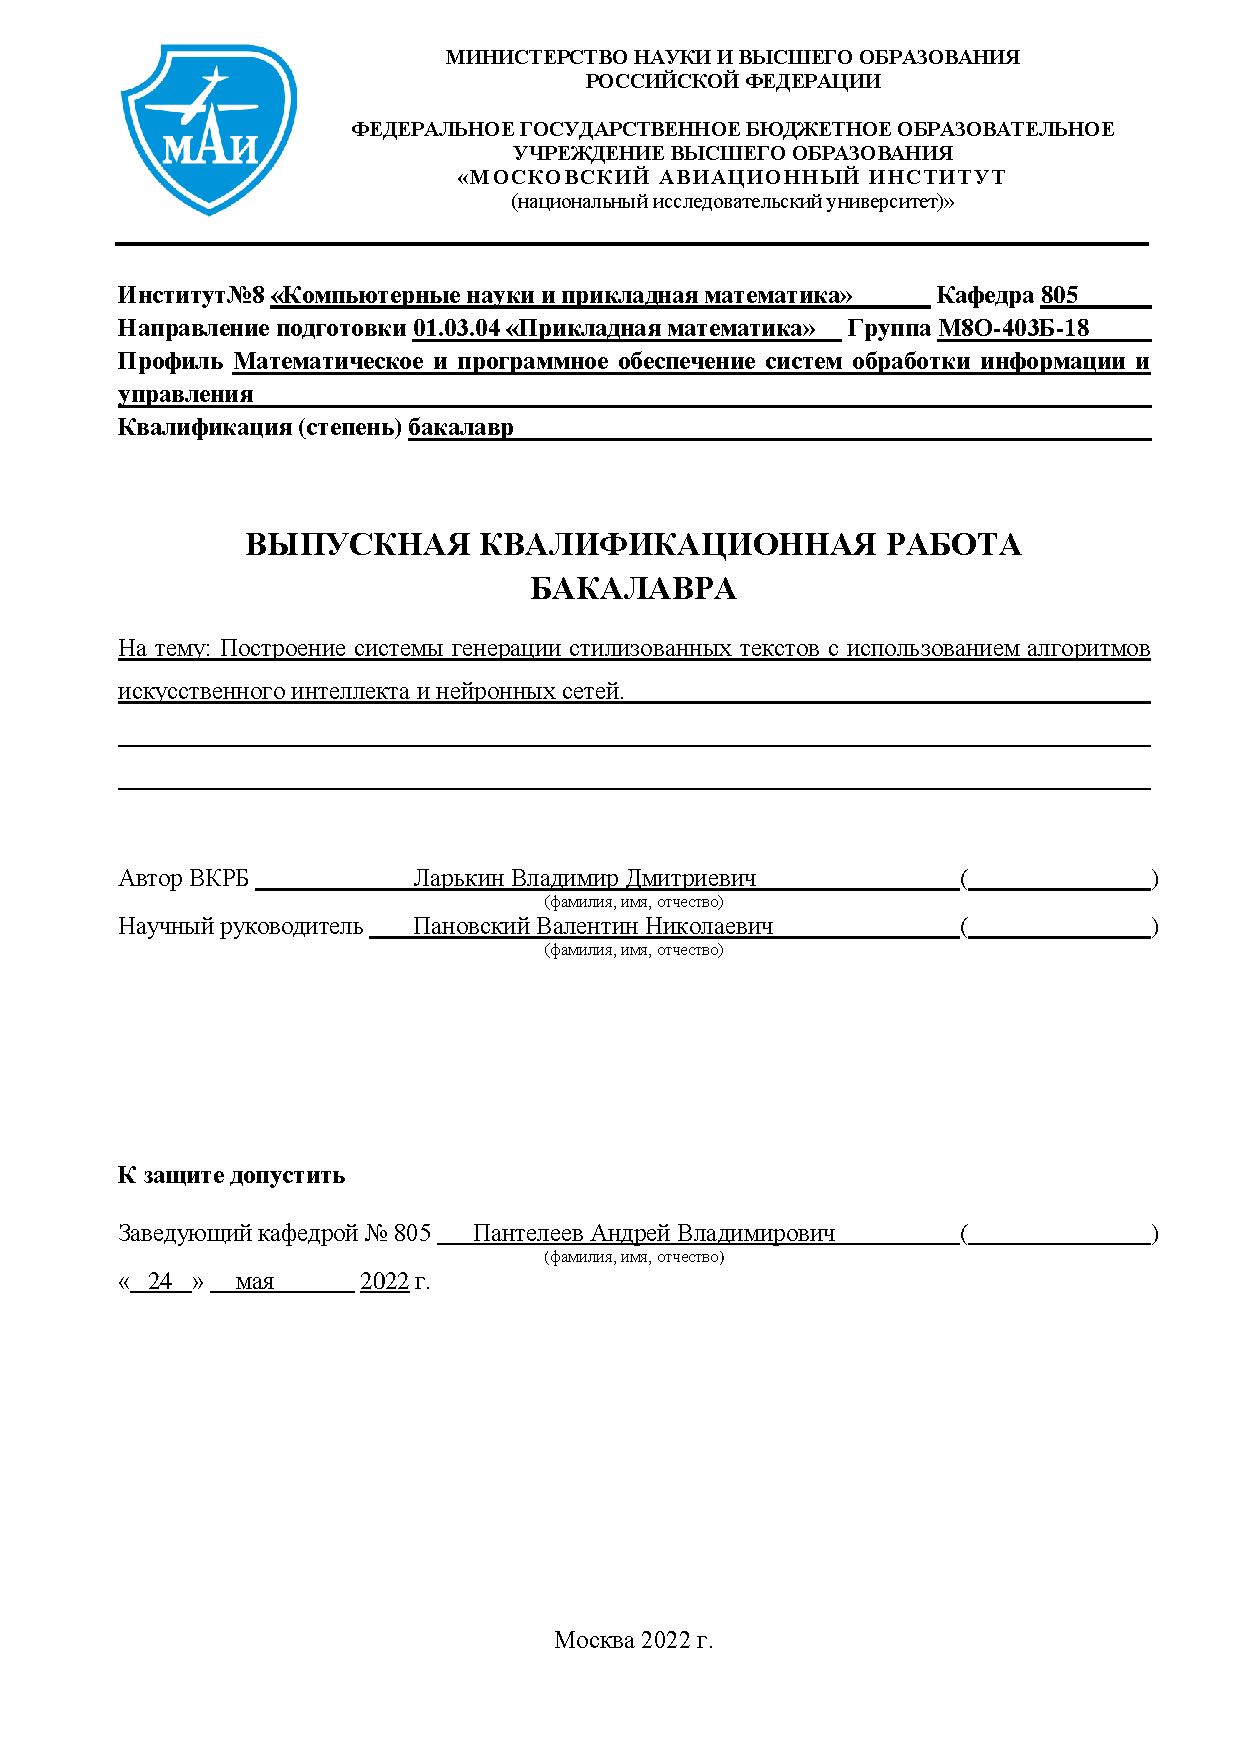
\includepdf[pages=-]{../inc/title.pdf}

% Также можно использовать \Referat, как в оригинале
\setcounter{page}{2}
\begin{abstract}

    Отчет содержит \pageref{LastPage}\,стр.%
    \ifnum \totfig >0
    , \totfig~рис.%
    \fi
    \ifnum \tottab >0
    , \tottab~табл.%
    \fi
    %
    \ifnum \totbib >0
    , \totbib~источн.%
    \fi
    %
    \ifnum \totapp >0
    , \totapp~прил.%
    \else
    .%
    \fi

    ГЕНЕРАЦИЯ ТЕКСТА, НЕЙРОННЫЕ СЕТИ, NLP, TRANSFORMER, ДООБУЧЕНИЕ, RUGPT-3

    В работе представлено решение задачи дообучения языковой модели архитектуры Transformer для генерации стилизованного текста из заданной предметной области.

\end{abstract}


\tableofcontents

\printnomenclature % Автоматический список сокращений

\Introduction
\label{cha:intro}

\blindtext \cite{gh:sber}
\vspace*{\fill}
\addcontentsline{toc}{chapter}{Основная часть}
\begin{center}
    \bfseries\MakeUppercase{Основная часть}
\end{center}
\label{cha:main}
\vspace*{\fill}

\mainmatter % это включает нумерацию глав и секций в документе ниже

\chapter{Теоретическая часть}
\label{cha:theory}

\section{Определения}

\textbf{Корпус текстов} --- множество подобранных и определённым образом обработанных текстов.

\textbf{Токен} --- элементарная единица разбиения корпуса.

\textbf{Токенизация} --- процесс разбиения корпуса на токены с присвоением им уникальных числовых идентификаторов.

\textbf{Языковая модель} --- распределение $P(w_t | w_1,w_2,w_3,\dots,w_n)$ вероятностей встретить токен $w_t$ в корпусе сразу после $n$ токенов $w_i$, $i\in[1, n]$, идущих подряд, где $w_i \in W \, \forall i$, $W$ --- множество всех токенов корпуса, $n$ --- длина контекста модели.

\textbf{Длина контекста} --- количество $n$ токенов $w_i$, $i\in[0, n]$, предшествующих токену $w_t$, от которых зависит вероятность появления в тексте токена $w_t$.

\textbf{Дообучение} --- процесс обучения уже обученной на некоторых данных модели машинного обучения на новых данных. В случае языковой модели это означает подстройку модели под новое распределение токенов.

\textbf{Перплексия} --- мера схожести двух вероятностных распределений, используемая для оценки качества генерации текста языковой моделью. Перплексия задаётся формулой \ref*{eq:perplexity}.
\begin{equation}
    \label{eq:perplexity}
    \textrm{PP}(W)=\sqrt[n]{\frac{1}{P(w_1,w_2,\dots,w_n)}}
\end{equation}

\section{Постановка задачи}

Заданы:
\begin{itemize}
    \item корпус, состоящий из текстов, принадлежащих конкретной предметной области,
    \item предобученная нейросетевая языковая модель, хорошо моделирующая вероятностное распределение слов в естественном языке.
\end{itemize}
Требуется: дообучить данную языковую модель на данных из корпуса, получив новую языковую модель, моделирующую распределение вероятностей слов в данном корпусе, и применить её для генерации новых текстов, принадлежащих предметной области данного корпуса, встроив в графический пользовательский интерфейс.


\backmatter %% Здесь заканчивается нумерованная часть документа и начинаются ссылки и
            
\Conclusion
\label{cha:conclusion}

В результате выполнения описанной работы были решены следующие подзадачи:
\begin{itemize}
    \item найден и предобработан корпус --- набор сценариев юмористических телешоу,
    \item выбрана и дообучена предобученная нейросетевая языковая модель ruGPT-3 Small архитектуры Transformer с использованием библиотек для глубокого обучения PyTorch и Transformers для языка Python,
    \item разработан графический веб-интерфейс с использованием фреймворка Streamlit на Python, предоставляющий следующие возможности:
    \begin{itemize}[$\bullet$]
        \item дополнение введённого пользователем текста сгенерированным нейронной сетью,
        \item отмена результатов генерации,
        \item свободное редактирование получившегося документа,
        \item сохранение результата на компьютере,
    \end{itemize}
    \item приложение для упрощения дистрибуции упаковано в изолированное окружение --- контейнер, созданный при помощи технологии Docker.
\end{itemize}

По итогу проделанной работы можно заключить, что все изначально поставленные задачи были успешно выполнены:
\begin{itemize}
    \item сгенерированные моделью тексты по форме действительно являются сценариями юмористических телешоу: они имеют аналогичную структуру, а при прочтении человеком могут вызвать у него смех,
    \item графический интерфейс получился удобным для взаимодействия с моделью, предоставляет достаточно гибкие возможности для экспериментов,
    \item технология Docker как средство упаковки приложения оказала положительное влияние на простоту развёртывания приложения на локальном компьютере, позволив прописать чёткие и универсальные инструкции для пользователя.
\end{itemize}
%% заключение


\bibliographystyle{ugost2008}
\bibliography{thesis}



\appendix   % Тут идут приложения

\chapter{Листинги исходного кода}
\label{cha:appendix1-listing}

\lstinputlisting[language=Python, caption={Графический интерфейс пользователя}, label=lst:demo]{../inc/code/demo.py}
\lstinputlisting[language=Python, caption={Модуль генерации текста}, label=lst:generate]{../inc/code/generate.py}
\lstinputlisting[language=Python, caption={Скрипт для валидации и обработки данных}, label=lst:humanize]{../inc/code/humanize_data.py}


\end{document}

%%% Local Variables:
%%% mode: latex
%%% TeX-master: t
%%% End:
